\graphicspath{{content/1_literatureReview/figures/}}
\section{Lead-Acid Batteries}

Lead-acid battery cells permit a range of charging voltages. The voltage values are dependent on a number of factors, namely how the battery will be used,
the ambient temperature, the stage in the charging cycle, and, of course, the number of cells.

If the battery is to be used regularly, it is said to be in "cycle" mode and should be charged at the "cycle" voltage. "Standby" or "floating" voltage levels
are also possible for prolonged life and less regular use-cases. The ambient temperature also influences the desired voltage, with hotter temperatures
requiring lower charge voltages.

\begin{figure}[!htb]
  \centering
  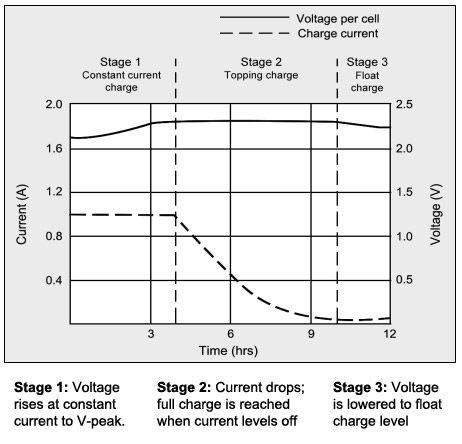
\includegraphics[width=0.4\textwidth]{batteryCharging_stages}
  \caption{The 3 Charging Stages for Lead-Acid Batteries}
  \label{fig:batteryCharging_stages}
\end{figure}

\noindent
These batteries should be charged in a three-stage process \cite{leadAcidCharging}, as seen in Figure \ref{fig:batteryCharging_stages}.
For stage 1 and 2, the cycle voltage is applied until the current reduces to a small value. In stage 3, the slightly lower "float" voltage should then be applied.
This helps keep the battery at a high enough voltage to prevent damage due to self-discharge.

Charging voltages are typically specified "per-cell". A typical cycle voltage is between $2.40$ and $\SI{2.45}{V \cdot cell^{-1}}$, while a typical float voltage is
between $2.30$ and $\SI{2.35}{V \cdot cell^{-1}}$ \cite{leadAcidCharging}. Charging currents may be chosen based on lifetime requirements, however most manufacturers
recommend a limit of $\SI{0.3}{C}$ or 0.3 times the rated capacity of the battery. Slightly higher currents may be allowed while the cells are still at low capacity,
and slightly lower currents may be used to prolong the life of the battery. During float-charging, the battery typically draws around 0.001C \cite{leadAcidCharging2}.

The RT670 supplied for this project has 3 cells and can charge at a cycle voltage of between $7.30$ to $\SI{7.40}{V}$ i.e. around $\SI{2.45}{V \cdot cell^{-1}}$ \cite{datasheetBattery}.
Its technical maximum charging current is $\SI{2.10}{A}$ and, since its capacity is $\SI{7}{Ah}$, this indicates a charge rating of $\SI{0.3}{C}$ as expected. The RT640, also supplied for this
project, has similar specifications, except permits a charging current of $\SI{1.2}{A}$ and a slightly wider cycle voltage range.